
% !TeX spellcheck = de_DE

\documentclass{article}

\usepackage[ngerman]{babel}
\usepackage{graphicx}
\usepackage{indentfirst}
\usepackage{hyperref}
\usepackage{geometry}
\usepackage{changepage}
\usepackage{booktabs}
\usepackage{float}
\usepackage{tabulary}
\usepackage{xcolor}
\usepackage{multirow}
\usepackage{caption}
\usepackage{subcaption}
\usepackage{lscape}
\usepackage{colortbl}
\usepackage{listings}
\usepackage[normalem]{ulem}
\usepackage{longtable}

\graphicspath{ {./images/} }
\setlength\parindent{0pt}

\makeatletter
\newcommand{\sectionauthor}[1]{
	{\parindent 0em \large \scshape Autor: #1 \par \nobreak \vspace*{1em}}
	\@afterheading
}
\makeatother

\title{Bibliotheksanwendung - Feinspezifikation}
\date{\today\\v1.1}
\author{
	Ivan Charviakou\\
	León Liehr\\
	Mohamad Najjar\\
	Jonas Picker\\
	Sergei Pravdin
}

\begin{document}
\maketitle
\begin{figure}[H]
	\centering
	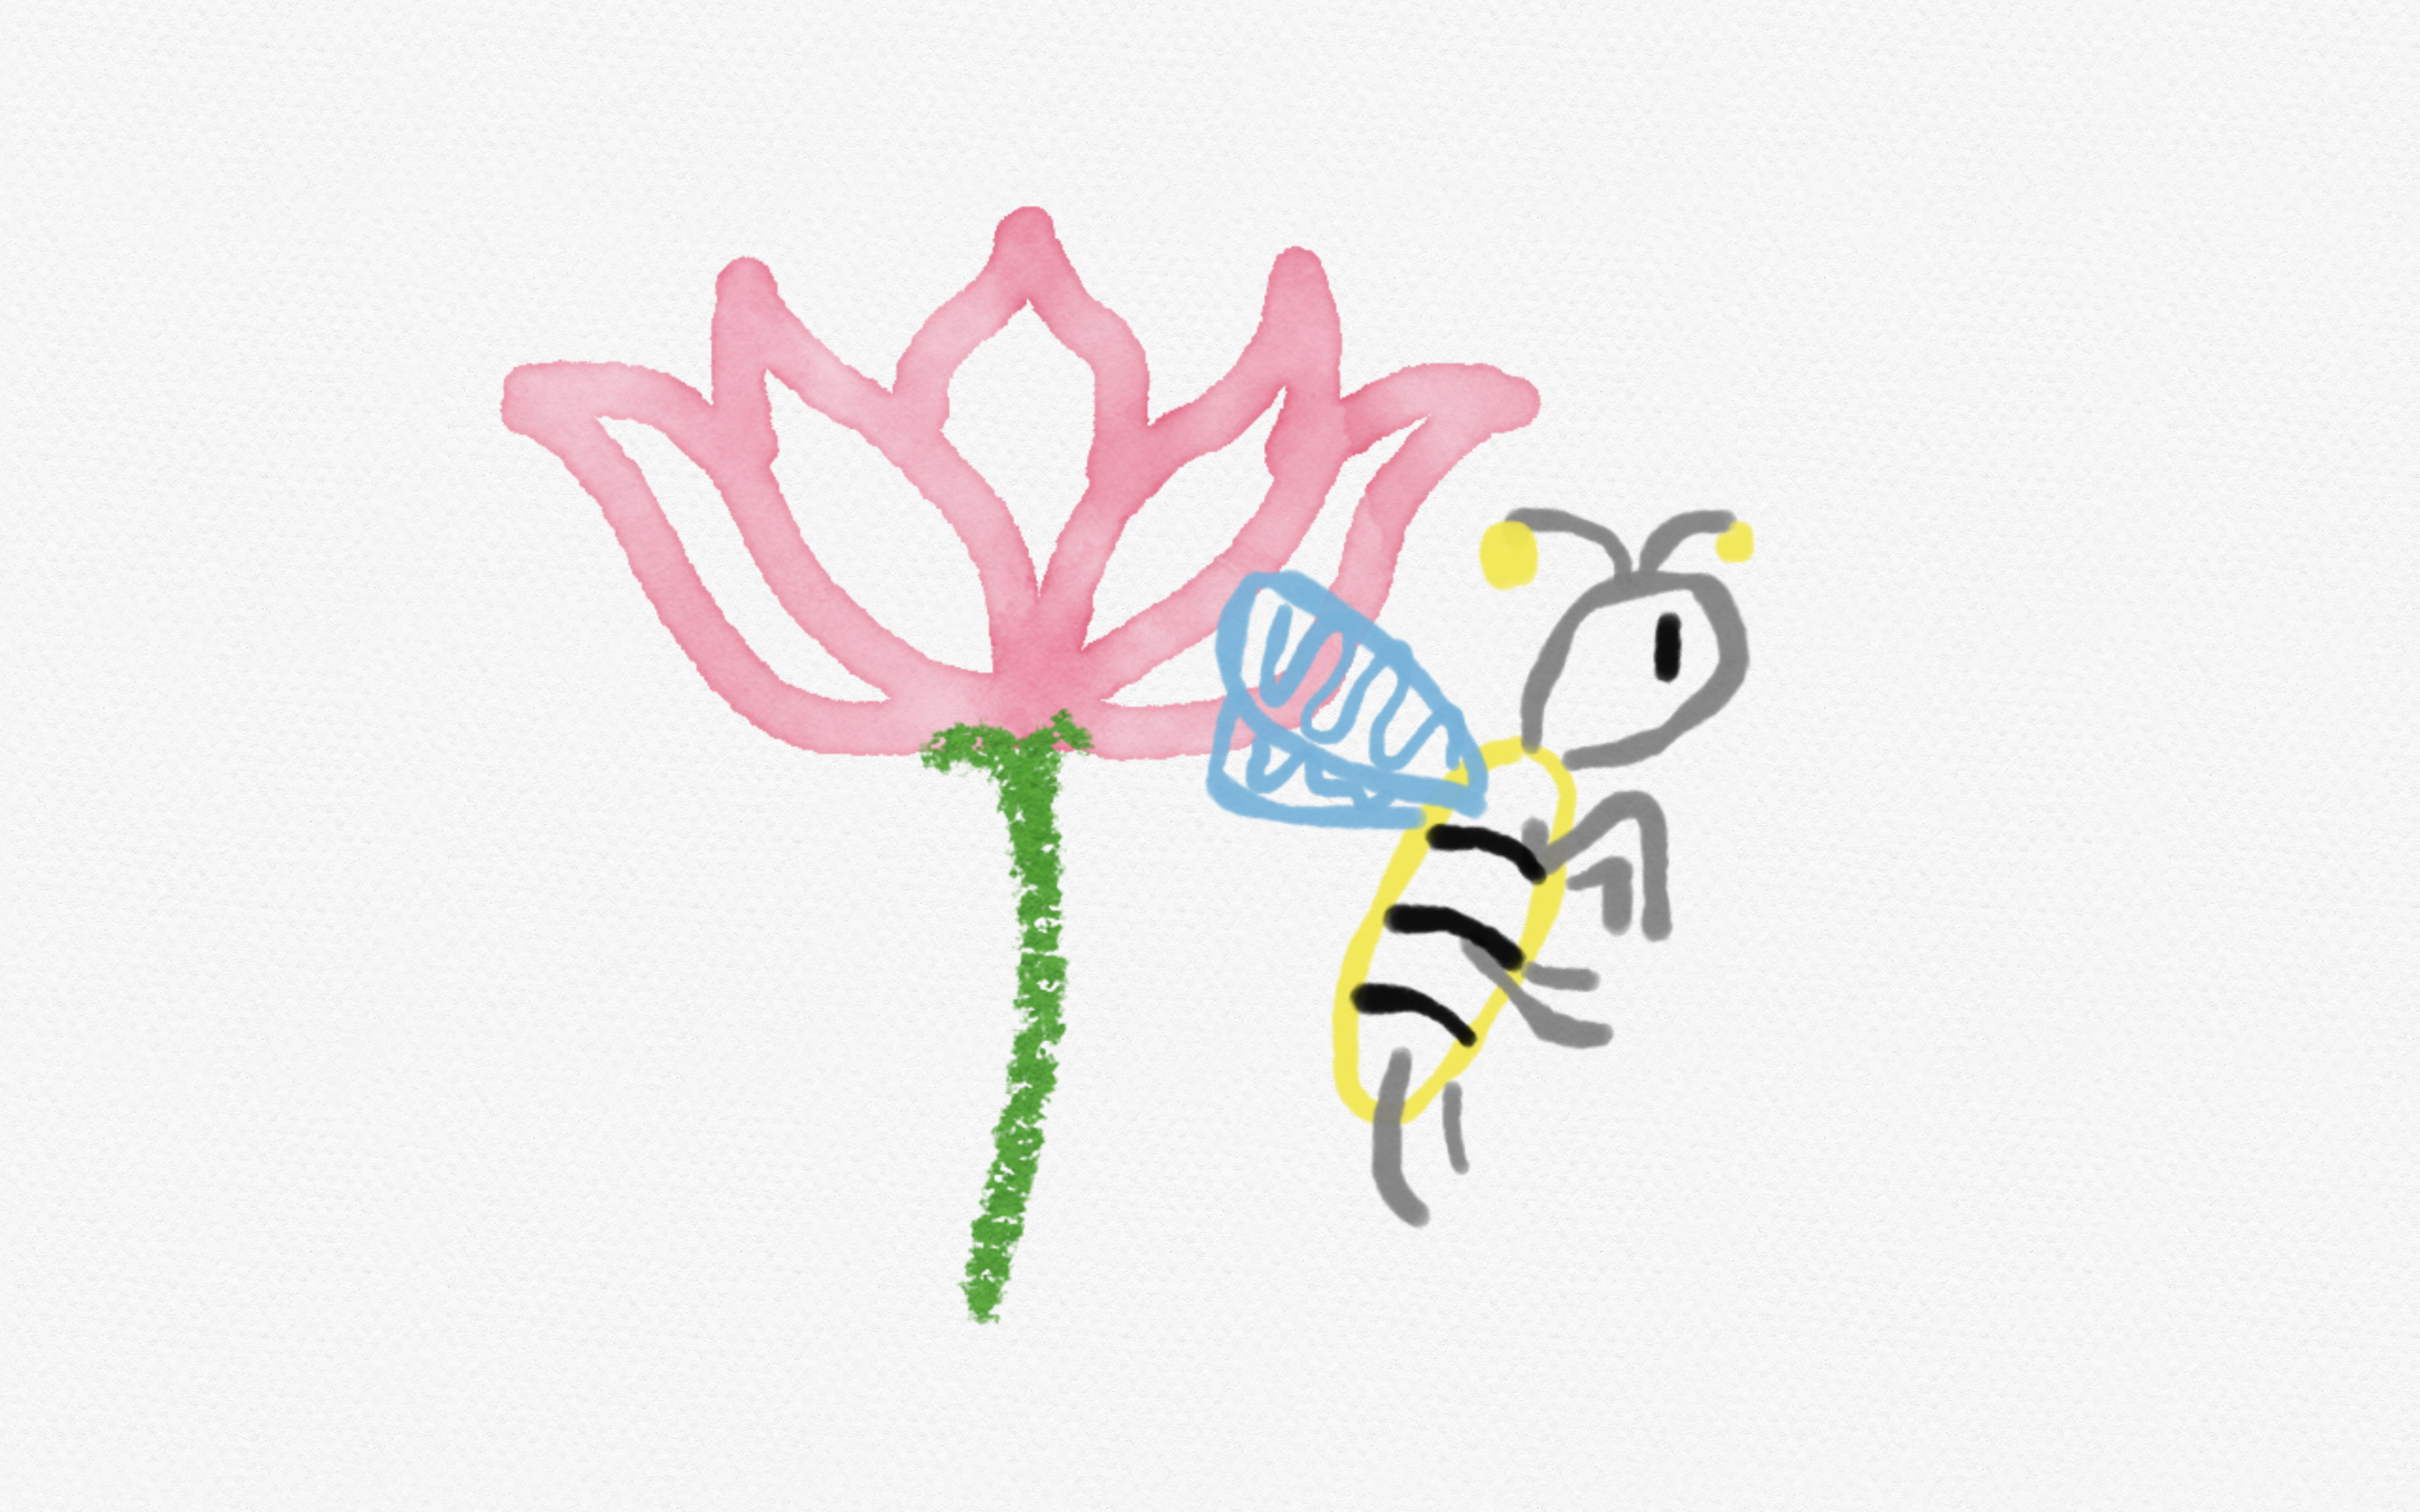
\includegraphics[width = 30em]{Logo}
\end{figure}
\newpage
\tableofcontents
\newpage

%----------------------------------------------------------------------Kapitel 1--------------------------------------------------------------------------------------------

\section{Milestones}

%----------------------------------------------------------------------Kapitel 2--------------------------------------------------------------------------------------------

\section{Arbeitspakete}

Die folgenden Tabellen geben unter Anderem die Klassen, Methoden, und Facelets an, die verschiedenen Arbeitspaketen innerhalb von Milestones zugeordnet sind. 
Dabei entsprechen die Tabellen den drei Milestones, die im Projekt vorgesehen sind.

\subsection{Milestone 2}
\sectionauthor{Ivan Charviakou}

\begin{longtable}{|l|l|l|l|} 
\hline
\textbf{\uline{Arbeitspaket / Element}} & \textbf{\uline{ID / Inhalt}}             & \textbf{\uline{Bearbeiter}} & \textbf{\uline{Zeit}}  \endfirsthead 
\hline
\textit{\textbf{Nutzerprofil}}          & \textit{\textbf{120}}                    & \textit{\textbf{Mohamad}}   & \textit{\textbf{3}}    \\ 
\hline
Facelet: Profilseite                    & profile.xhtml                            &                             &                        \\ 
\hline
Backing-Bean: Profilseite               & Profile.init()                           &                             &                        \\ 
\hline
                                        & Profile.user                             &                             &                        \\ 
\hline
                                        & Profile.password                         &                             &                        \\ 
\hline
                                        & Profile.confirmedPassword                &                             &                        \\ 
\hline
                                        & Profile.delete()                         &                             &                        \\ 
\hline
                                        & Profile.save()                           &                             &                        \\ 
\hline
Session-Bean: Nutzer                    & UserSession.user                         &                             &                        \\ 
\hline
DAO: Nutzer                             & UserDao.updateUser(…)                    &                             &                        \\ 
\hline
                                        & UserDao.deleteUser(…)                    &                             &                        \\ 
\hline
\textit{\textbf{Medienerstellung}}      & \textit{\textbf{80}}                     & \textit{\textbf{Ivan}}      & \textit{\textbf{5}}    \\ 
\hline
Facelet: Medienerstellung               & medium-creator.xhtml                     &                             &                        \\ 
\hline
Backing-Bean: Medienerstellung          & MediumCreator.init()                     &                             &                        \\ 
\hline
                                        & MediumCreator.medium                     &                             &                        \\ 
\hline
                                        & MediumCreator.copy                       &                             &                        \\ 
\hline
                                        & MediumCreator.user                       &                             &                        \\ 
\hline
                                        & MediumCreator.createMedium()             &                             &                        \\ 
\hline
DTO: Medium                             & MediumDto.id                             &                             &                        \\ 
\hline
                                        & MediumDto.category                       &                             &                        \\ 
\hline
                                        & MediumDto.returnPeriod                   &                             &                        \\ 
\hline
                                        & MediumDto.getAttribute(…)                &                             &                        \\ 
\hline
                                        & MediumDto.setAttribute(…)                &                             &                        \\ 
\hline
                                        & MediumDto.getCopy(…)                     &                             &                        \\ 
\hline
                                        & MediumDto.setCopy(…)                     &                             &                        \\ 
\hline
DAO: Medium                             & MediumDao.createMedium(...)              &                             &                        \\ 
\hline
                                        & MediumDao.createCopy(...)                &                             &                        \\ 
\hline
\textbf{\textit{Medienattribute}}       & \textbf{\textit{81}}                     & \textbf{\textit{Jonas}}     & \textbf{\textit{5}}    \\ 
\hline
Facelet: Medienschema                   & medium-schema-editor.xhtml               &                             &                        \\ 
\hline
Backing-Bean: Medienschema              & MediumSchemaEditor.init()                &                             &                        \\ 
\hline
                                        & MediumSchemaEditor.addAttribute()        &                             &                        \\ 
\hline
                                        & MediumSchemaEditor.deleteAttribute(...)  &                             &                        \\ 
\hline
                                        & MediumSchemaEditor.save()                &                             &                        \\ 
\hline
DTO: Attribut                           & AttributeDto.id                          &                             &                        \\ 
\hline
                                        & AttributeDto.name                        &                             &                        \\ 
\hline
                                        & AttributeDto.textValue                   &                             &                        \\ 
\hline
                                        & AttributeDto.imageValue                  &                             &                        \\ 
\hline
                                        & AttributeDto.urlValue                    &                             &                        \\ 
\hline
                                        & AttributeDto.attributeModifiability      &                             &                        \\ 
\hline
                                        & AttributeDto.type                        &                             &                        \\ 
\hline
                                        & AttributeDto.attributeMultiplicity       &                             &                        \\ 
\hline
                                        & AttributeDto.position                    &                             &                        \\ 
\hline
DAO: Medium                             & MediumDao.updateGlobalAttributes(...)    &                             &                        \\ 
\hline
                                        & MediumDao.readGlobalAttributes()         &                             &                        \\ 
\hline
\textbf{\textit{Mediumansicht I}}       & \textbf{\textit{83}}                     & \textbf{\textit{Sergei}}    & \textbf{\textit{5}}    \\ 
\hline
Facelet: Mediumansicht                  & medium.xhtml                             &                             &                        \\ 
\hline
Backing-Bean: Mediumansicht             & Medium.init()                            &                             &                        \\ 
\hline
                                        & Medium.saveAttributes()                  &                             &                        \\ 
\hline
                                        & Medium.createCopy()                      &                             &                        \\ 
\hline
                                        & Medium.deleteCopy()                      &                             &                        \\ 
\hline
                                        & Medium.medium                            &                             &                        \\ 
\hline
                                        & Medium.copy                              &                             &                        \\ 
\hline
DTO: Exemplar                           & CopyDto.id                               &                             &                        \\ 
\hline
                                        & CopyDto.location                         &                             &                        \\ 
\hline
                                        & CopyDto.signature                        &                             &                        \\ 
\hline
                                        & CopyDto.deadline                         &                             &                        \\ 
\hline
                                        & CopyDto.copyStatus                       &                             &                        \\ 
\hline
                                        & CopyDto.actor                            &                             &                        \\ 
\hline
DAO: Medium                             & MediumDao.readCopy(...)                  &                             &                        \\ 
\hline
                                        & MediumDao.updateMediumAttributes(…)      &                             &                        \\ 
\hline
\textbf{\textit{Mediumansicht II}}      & \textbf{\textit{82}}                     & \textbf{\textit{Mohamad}}   & \textbf{\textit{5}}    \\ 
\hline
Backing-Bean: Mediumansicht             & Medium.getReturnPeriod()                 &                             &                        \\ 
\hline
                                        & Medium.updateReturnPeriod()              &                             &                        \\ 
\hline
                                        & Medium.saveCopy()                        &                             &                        \\ 
\hline
                                        & Medium.lendCopy()                        &                             &                        \\ 
\hline
                                        & Medium.returnCopy()                      &                             &                        \\ 
\hline
                                        & Medium.pickUpCopy()                      &                             &                        \\ 
\hline
                                        & Medium.cancelPickup()                    &                             &                        \\ 
\hline
DAO: Medium                             & MediumDao.updateCopy(...)                &                             &                        \\ 
\hline
                                        & MediumDao.deleteCopy(...)                &                             &                        \\ 
\hline
\textbf{\textit{Kategoriesuche}}        & \textbf{\textit{110}}                    & \textbf{\textit{Leon}}      & \textbf{\textit{4}}    \\ 
\hline
Facelet: Kategoriesuche                 & category-browser.xhtml                   &                             &                        \\ 
\hline
Backing-Bean: Kategoriesuche            & CategoryBrowser.init()                   &                             &                        \\ 
\hline
                                        & CategoryBrowser.categorySearch           &                             &                        \\ 
\hline
                                        & CategoryBrowser.currentCategory          &                             &                        \\ 
\hline
                                        & CategoryBrowser.deleteCategory()         &                             &                        \\ 
\hline
                                        & CategoryBrowser.searchCategory()         &                             &                        \\ 
\hline
                                        & CategoryBrowser.getItems()               &                             &                        \\ 
\hline
DTO: Kategoriensuche                    & CategorySearchDto.searchTerm             &                             &                        \\ 
\hline
DAO: Kategorie                          & CategoryDao.readCategory()               &                             &                        \\ 
\hline
                                        & CategoryDao.readCategoriesByName()       &                             &                        \\ 
\hline
\textbf{\textit{Kategorieerstellung}}   & \textbf{\textit{111}}                    & \textbf{\textit{Leon}}      & \textbf{\textit{4}}    \\ 
\hline
Facelet: Kategorieerstellung            & category-creator.xhtml                   &                             &                        \\ 
\hline
Backing-Bean: Kategorieerstellung       & CategoryCreator.init()                   &                             &                        \\ 
\hline
                                        & CategoryCreator.category                 &                             &                        \\ 
\hline
                                        & CategoryCreator.createCategory()         &                             &                        \\ 
\hline
DTO: Kategorie                          & CategoryDto.id                           &                             &                        \\ 
\hline
                                        & CategoryDto.name                         &                             &                        \\ 
\hline
                                        & CategoryDto.description                  &                             &                        \\ 
\hline
                                        & CategoryDto.parent                       &                             &                        \\ 
\hline
DAO: Kategorie                          & CategoryDao.createCategory(…)            &                             &                        \\ 
\hline
                                        & CategoryDao.updateCategory(…)            &                             &                        \\ 
\hline
                                        & CategoryDao.deleteCategory(…)            &                             &                        \\ 
\hline
\textbf{\textit{Medientransaktionen}}   & \textbf{\textit{90}}                     & \textbf{\textit{Sergei}}    & \textbf{\textit{4}}    \\ 
\hline
Facelet: Medienausleihe                 & lending.xhtml                            &                             &                        \\ 
\hline
Backing-Bean: Medienausleihe            & Lending.init()                           &                             &                        \\ 
\hline
                                        & Lending.user                             &                             &                        \\ 
\hline
                                        & Lending.copies                           &                             &                        \\ 
\hline
                                        & Lending.lendCopies()                     &                             &                        \\ 
\hline
                                        & Lending.addSignatureInputField()         &                             &                        \\ 
\hline
Facelet: Medienrückgabe                 & return-form.xhtml                        &                             &                        \\ 
\hline
Backing-Bean: Medienrückgabe            & ReturnForm.init()                        &                             &                        \\ 
\hline
                                        & ReturnForm.user                          &                             &                        \\ 
\hline
                                        & ReturnForm.copies                        &                             &                        \\ 
\hline
                                        & ReturnForm.returnCopies()                &                             &                        \\ 
\hline
                                        & ReturnForm.addSignatureInputField()      &                             &                        \\ 
\hline
DAO: Medium                             & MediumDao.lendCopy(...)                  &                             &                        \\ 
\hline
                                        & MediumDao.returnCopy(...)                &                             &                        \\ 
\hline
\textbf{\textit{Wartungsprozess}}       & \textbf{\textit{170}}                    & \textbf{\textit{Jonas}}     & \textbf{\textit{3}}    \\ 
\hline
Klasse: Wartungsprozess                 & MaintenanceProcess.setTimeoutInterval(…) &                             &                        \\ 
\hline
                                        & MaintenanceProcess.run()                 &                             &                        \\ 
\hline
                                        & MaintenanceProcess.shutdown()            &                             &                        \\ 
\hline
\textbf{\textit{Trespasslistener}}      & \textbf{\textit{161}}                    & \textbf{\textit{Ivan}}      & \textbf{\textit{3}}    \\ 
\hline
Klasse: Trespasslistener                & TrespassListener.beforePhase(…)          &                             &                        \\ 
\hline
                                        & TrespassListener.afterPhase(…)           &                             &                        \\ 
\hline
                                        & TrespassListener.getPhaseId()            &                             &                        \\
\hline
\end{longtable}



%----------------------------------------------------------------------Kapitel 3--------------------------------------------------------------------------------------------

\section{PERT-Diagramm}
\sectionauthor{Ivan Charviakou}

Im Folgenden wird das PERT Diagramm zum Projekt dargestellt. Insbesondere bildet es die Abhängigkeiten zwischen den Paketen ab und zeigt das kritische Pfad im Projekt auf. Dabei werden die Zeitdauer in Stunden berechnet.

\begin{figure}[H]
	\centering
	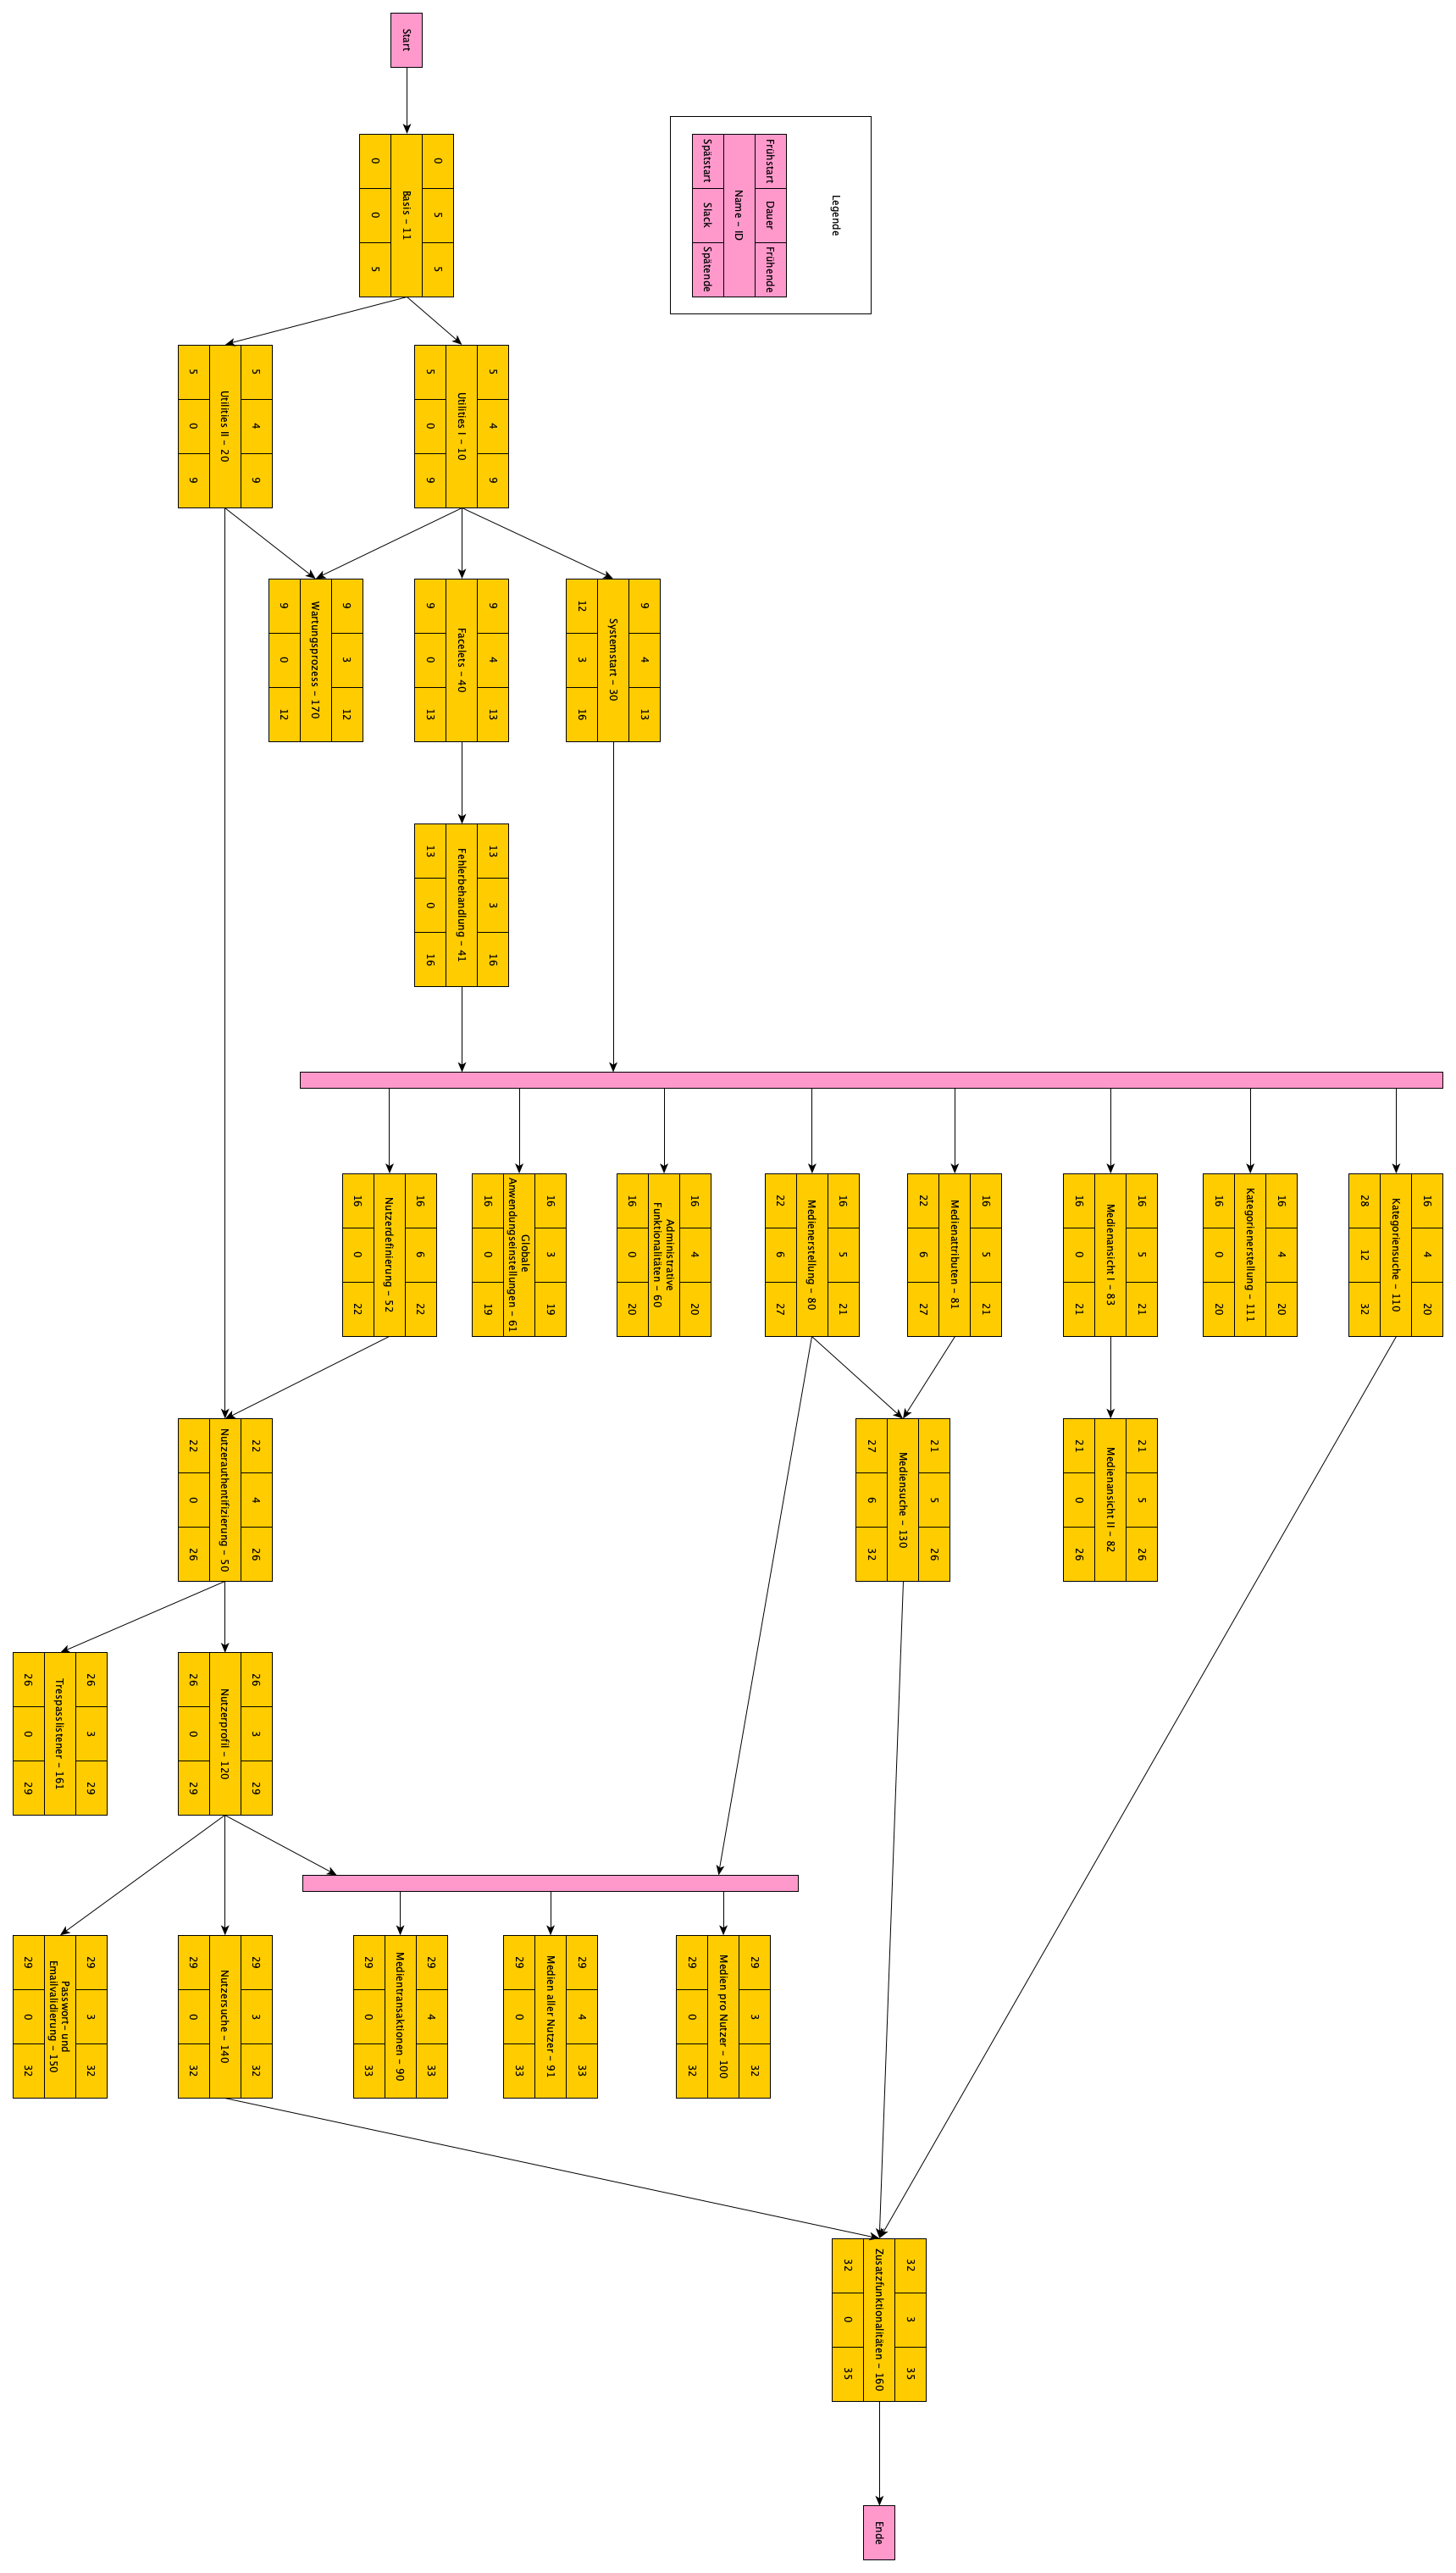
\includegraphics[width = 30em]{PERT}
\end{figure}

%----------------------------------------------------------------------Kapitel 4--------------------------------------------------------------------------------------------

\section{Spezialgebiete}

%----------------------------------------------------------------------Kapitel 5--------------------------------------------------------------------------------------------

\section{Whitebox-Tests}


\end{document}
